\chapter{Lecture}\label{lec3}%chap 3

\setcounter{section}{1}
\section{Spaces \texorpdfstring{$H^m$}{Hm}}\pageoriginale\label{lec3:sec2} %sec 2.

\subsection{}\label{lec3:sec2:subsec1}

\begin{definition}\label{lec3:sec2:subsec1:def2.1}%defi 2.1
$u \in H^m (\Omega) \Leftrightarrow D^p u \in L^2
  (\Omega)$ for $|p|\le m [D^o u=u]$. Hence $H^m (\Omega) = H (A;
  \Omega)$, where  $A= \{ D^p, |p|\le m \}$. If we write $|u|^2_k=
  \sum \limits _{|p|=k}|D^pu|^2_o$ and $\parallel u \parallel ^2_m
  =\sum\limits_{k \leq m} |u|^2_k$, then the norm in $H^m(\Omega)$ is
  $\parallel u \parallel _m$. 
\end{definition}

By theorem \ref{lec1:sec1:subsec2:thm1.1} and propositions \ref{lec2:sec1:subsec6:prop1.5} and \ref{lec1:sec1:subsec4:prop1.3}, we have   
\begin{theorem}\label{lec3:sec2:subsec1:thm2.1}%theo 2.1
$H^m(\Omega)$ is a Hilbert space. In order that a distribution $T$ on
  $\Omega$ belongs to $H'^m_o(\Omega)$ it is necessary and sufficient
  that $T = \sum\limits_{|p|\le m} D^p f_p$ for $f_p \in L^2
  (\Omega)$. 
\end{theorem}

We shall write $H_o^m(\Omega) = H^{-m}(\Omega)$.

\begin{proposition}\label{lec3:sec2:subsec1:prop2.1}%prop 2.1
  $u \in H^m (R^n)$, if and only if $\hat{u} \in L^2$
  and $\xi^p \hat{u} \in L^2$ for $|p|\le m$. Or equivalently,
  if and only if $(1+|\xi|^m) \hat{u} \in L^2$ where $|\xi|^2
  = \xi^2_1+ \cdots + \xi ^2_n$. 
\end{proposition}

Regarding the local nature of $H^m (\Omega)$, we have the 
\begin{proposition}\label{lec3:sec2:subsec1:prop2.2}%prop 2.2
  Let $u \in H^m (\Omega)$ (respectively $H^m_o (\Omega)$) and
  $\varphi \in \mathscr{D}(\Omega)$. Then $(i)\varphi u
  \in H^m (\Omega)$ (respectively $H^m_o (\Omega)$), $(ii) u \to
  \varphi. u$ is a continuous mapping from $H^m (\Omega)$ to
  $H^m(\Omega)$ (respectively $H^m_o (\Omega)$ to $H^m_o(\Omega)$). 
\end{proposition}

This theorem holds actually with $\varphi \in L^ \infty
(\Omega)$ such that $D^p \varphi \in L^\infty$ for $|p|\le
m$. 

Let $X$ be a closed set in $R^n$. Write $H^{-m}_X= \{ T \in
H^{-m}(R^n)$ such that the support of $T \subset X \}$. 

\begin{definition}\label{lec3:sec2:subsec1:def2.2}%defin 2.2
  $X$\pageoriginale is said to be $m$-polar if $H^{-m}_X=0$, i.e., if they only
  distribution of $H^{-m}(R^n)$ with support in $X$ is $0$.  
\end{definition}

We shall see later that if $2m > n, X$ is void. We shall admit, without proof,
\begin{theorem}\label{lec3:sec2:subsec1:thm2.2}%theo 2.2
  $H^m(\Omega)= H^m_o(\Omega)$ if and only if $[ \Omega$ is $m$- polar.
\end{theorem}

\subsection{Extension of functions in \texorpdfstring{$H_o(A; \Omega)$}{H0(A;Omega)} to \texorpdfstring{$R^n$}{Rn}}
\label{lec3:sec2:subsec2}  

\begin{definition}\label{lec3:sec2:subsec2:def2.3}%defini 2.3
  An open set $\Omega \subset R^n$ is said satisfy $m$-{\em extension
    property} if we can find a continuous linear mapping $\pi$ of $H^m
  (\Omega)$ to $H^m(R^n)$ such that $\pi u =u$ a.e. in $\Omega$. 
\end{definition}

\noindent 
\begin{minipage}{6cm}
  There are examples to show that not all $\Omega$ posses this
  property. For example in the case $m=1,n=2$ take the domain in the
  figure, which is an open square with the thickened line removed. Let
  $\underbar{u}$ be a function as indicated in the figure. Let $\varphi$
  be a $C^ \infty$ functions which vanishes outside the unit circle, is
  $1$ within a smaller circle and $0 \leq \varphi \le 1$ elsewhere. Then $v =
  \varphi u$ is zero on the boundary of the given square. We now prove
  that it is impossible to find to find $V$ such that $V=va.e$. on
  $\Omega$. For, if $V=v$, a.e. on $\Omega$, then 
\end{minipage}
\quad 
\begin{minipage}{4cm}
  \begin{figure}[H]
    \centering{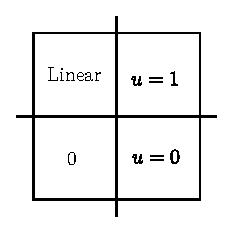
\includegraphics{vol10-figures/fig10-chap3-1.eps}}
  \end{figure}
\end{minipage}
\begin{equation*}
  \frac{\partial v}{\partial y}=
  \begin{cases}
    \text{ sometimes outside } \Omega.\\ 
    \frac{\partial \varphi}{\partial
      y}u + \varphi \frac{\partial u}{\partial y} \text { in } \Omega. 
  \end{cases}
\end{equation*}

Now $\dfrac{\partial u}{\partial y}$ is a measure supported by th
thickened line. Hence $\dfrac{\partial V}{\partial y}$ is not a
function. 

However, in the following two theorems, it will be proved that some
usual domains posses the $m$-extension property. 

\begin{theorem}\label{lec3:sec2:subsec2:thm2.3}%theo 2.3 
  Let\pageoriginale $\Omega = \{ x_n >0 \} =R^+_n$. Then $\Omega$ has $m$-extension
  property for any $\underbar{m}$. 
\end{theorem}

Let $\mathscr{D}(\bar{\Omega})$ be the restrictions of functions of
$\mathscr{D}(R^n)$ to $\Omega$. We require the following 
\begin{lemma*}
  $H^m (\Omega)\cup \mathscr{D}(\bar{\Omega})$ is dense in $H^m (\Omega)$.
\end{lemma*}

Assume for the time being this lemma, we shall first complete the
proof of the theorem \ref{lec3:sec2:subsec2:thm2.3}. It is enough to show that $\pi$ can be
defined continuously on $H^m(\Omega)\cap \mathscr{D}
(\bar{\Omega})$. We do this explicitly as follows: For $u \in
H^m (\Omega)\cap \mathscr{D}(\bar{\Omega})$, put 
\begin{equation*}
\pi (u(x)) \qquad =
     \begin{cases}
       u (x) &\text{ if } x_n \geq 0. \\ 
       \lambda _1  &u(x', -x_n) + \cdots +
       \lambda_m u(x',- \frac{x_n}{m})=v(x)\\ 
       & \text{ if } x_n <0. 
     \end{cases}
\end{equation*}
where $x' = (x_1, \ldots,x_{n-1})$.

We determine $\lambda_i$ in order to ensure that $\pi (u(x))
\in H^m (R^n)$. For that we need verify 
\begin{align*}
  &(v(x',0)=u(x',0), \qquad \text{i.e.} \lambda_1 + \cdots + \lambda_m =1. \\
  &\frac{\partial^{ m-1}v}{\partial^{m-1}x_n}(x',0)= \frac
  {\partial^{m-1}u}{\partial^{m-1}x_n}, ~\text{i.e.,}~ (-1)^{m-1^{\vdots}}
  (\lambda_1 +\cdots \frac{\lambda m}{m^{m-1}})=1. 
\end{align*}

These equations determine $\lambda'_1s$ and it is at once seen that
$D^p (\pi (u))=D^p u$ for $|p|\le m$, a.e, on $\Omega$ and
that  the mapping $\pi$ is continuous. 

Now we prove the lemma.

Let $u \in H^m(\Omega)$; for every $\in > 0$, define
$u_\epsilon (x)=u(x',x_n+\in)$. Let $v_\epsilon$ be the
restriction of $u_\epsilon $ to. It\pageoriginale is easy to see that $u_ \in
\to u$ in $H^m (\Omega)$ as $\in \to 0$, and so we need prove
only that $v_\epsilon$ for every fixed $\epsilon >0$ can be approximated by
functions of $H^m(\Omega) \cap \mathscr{D}(\bar{\Omega})$, i.e., we
have to prove that given a function $w \in H^m(\Omega
_\alpha)$, where $\omega _ \alpha$ is the domain $\{ x_n > - \alpha
\}, w$ can be approximated on $\Omega$ by functions of
$H^m(\Omega)\cap \mathscr{D} (\bar{\Omega})$. Let $\cup (x_n)$ be a
$C^ \infty$ function defined as follow: $\theta=0$ for $x_n < - \alpha,
1$ for $x_n >0,0< \theta <1$, elsewhere. Now $\theta w \in
H^m(R^n)$ and $\theta w=v$ a.e. in $\Omega$. However,
$\mathscr{D}(R^n)$ is dense in $H^m (R^n)$. Hence there exists a
sequences $\phi _k \in \mathscr{D}(R^n)$ such that $\phi \to
\theta w$ in $H^m (R^n)$. Let $\varphi _k$ be the restriction of $\phi
_k$ to $\Omega$. Then $\varphi _k \in H^m(\Omega) \cap
\mathscr{D} (\bar{\Omega})$ and $\varphi _k \to \theta w=w$ in
$H^m(\Omega)$. 

\begin{remark}\label{lec3:sec2:subsec2:rem1}%rema 1
  If $\Omega$ has $m$-extension property, then the above lemma holds,
  i.e., $H^m(\Omega) \cap \mathscr{D} (\bar{\Omega})$ is dense in
  $H^m(\Omega)$. For, since $\mathscr{D}$ is dense in $H^m(R^n)$, and
  since there exists a continuous mapping $\pi$ of $H^m(\Omega)$ in $H^m
  (R^n)$, the restrictions of functions of $\mathscr{D}$ to $\Omega$ are
  dense in $H^m(\Omega)$. 
\end{remark}

\begin{remark}\label{lec3:sec2:subsec2:rem2}%rema 2
  This lemma holds also, for instance, for star-shaped domains.
\end{remark}

\subsection{} \label{lec3:sec2:subsec3} %%% subsec3

\begin{theorem}\label{lec3:sec2:subsec3:thm2.4}%the 2.4
  Let $\Omega$ be an open bounded set such that the boundary of $\Omega$
  is an $(n-1)$ dimensional $C^m$ manifold $\Gamma \Omega$ lying on one
  side of $\Gamma$. Then $\Omega$ has the $m$-extension property. 
\end{theorem}

\begin{proof}
Let $\mathbb{Z}^n$ be the $m$-dimensional Euclidean space with
coordinates $\xi, \ldots , \xi_n$ and let $W$ be the open rectangle
define by 
$\begin{cases} 
0 < \xi_i <1 \\ 
-1 < \xi_n <1
\end{cases}
i=1, \ldots , n-1$.
Let $W_+,W_-,W_o$  denote the subsets of $W$ determined by $\xi >0,
\xi _n <0, \xi_n=0$, respectively. 
\end{proof}

On\pageoriginale account of the hypothesis on $\Gamma$, there exists a finite open covering
$O', O_i$ of $\bar{\Omega}$ and $m$-times continuously differentiable
functions $\psi _i$ of $W$ to $O_i$ such that $\psi_i$ maps $W_-$ onto
$O_i \cap \Gamma$, $W_+$ onto $O_i \cap [ \bar{\Omega}$ and $W_o$ onto
  $O_i \cap \Gamma$, and further, $O_i \cap \Gamma$ cover $\Gamma$ and
  Let $(a' ,a_i)$ be a $C^m$ partition of unity subordinate to this
  covering. If $u \in H^m (\Omega)$, then $u=a'u + \sum a_i u$
  and $a_i u$ have their supports in $O_i$ respectively. Now $\psi _i$
  defines an isomorphism of $H^m(O_i)$ onto $H^m(W)$ and of $H^m(0_i
  \cap \Omega)$ onto $H^m(W_-)$, which we still denote by
  $\psi_i$. Hence $v_i = \psi^{-1}_i (a_i u) \in H^m (W_-)$
  and $v_i=0$ near the part of the boundary of $W_-$ which is not
  contained in $\xi_n=0$. Hence $v_i$ can be extended to $(\xi_n <0)$
  by putting it equal to zero outside $W_-$. By theorem    \ref{lec3:sec2:subsec2:thm2.3}, there
  exists $\pi v_i \in H^m (\mathbb{Z}^n)$ such that $\pi v_i=v_i,
  a.e$. on $\mathbb{Z}^n$. Let $\theta (x_n)$ be a $C^\infty$ function
  which is $0$ for $\xi_n > \dfrac{2}{3}$ and $1$ for $\xi<
  \dfrac{1}{3},0 <\theta < 1$ elsewhere. Let $p(\xi)= \theta \pi
  (v_i)$. $P_i(\xi)$ has its support in $W$ and is zero near the
  boundary of $W$. Let $\varphi _i (x)=\psi_i(P)$. Then $\varphi (x)
  \in H^m(O_i)$ and is zero near the boundary of $O_i$. Hence
  $\pi (u)=a'_u+ \sum \tilde{ \varphi}_i (x)$ answers the
  theorem. 
